\documentclass[a4paper,12pt]{article}
\usepackage[utf8]{inputenc}
\usepackage[french]{babel}
\usepackage[T1]{fontenc}
\usepackage[margin=2.5cm]{geometry}
\usepackage{hyperref}
\usepackage{xcolor}
\definecolor{namecolour}{HTML}{0028BA}
\hypersetup{pdftitle=Documentation}
\newcommand{\tikzlg}{\href{https://ctan.org/pkg/tikz}{\color{black}Ti\textit{k}Z}}
\let\oldoplus\oplus
\usepackage{output/sffont,output/tools,output/htmlpreambule,output/matrices,output/al,output/bigoperators,output/analyse,output/arithmetique,output/dsft,output/equivalents,output/polynomes,output/probas,output/structures,output/trigo,output/tables,output/usuelles}
\usepackage[arc]{output/complexes}
\makeatletter
\newcommand{\oldl}{\lsb@l}
\makeatother
\SetSymbolFont{stmry}{bold}{U}{stmry}{m}{n}
\usepackage{minted}
\usemintedstyle{perso}
\setlength{\parindent}{0pt}
\setlength{\fboxsep}{0pt}
\hypersetup{hidelinks,colorlinks=true,linkcolor=black,linktoc=all,urlcolor=blue}
\setcounter{secnumdepth}{5}
\setcounter{tocdepth}{1}
\let\oldsection\section
\newcommand{\hsection}[1]{\clearpage\oldsection[#1]{\href{https://rfoxinter.github.io/revisions/output/#1}{\color{black}#1}}}
\newcommand{\ssection}[2][]{\clearpage\oldsection[#1]{#2}}
\title{\href{https://rfoxinter.github.io/revisions/Documentation.pdf}{\color{black}Documentation}\phantomsection\addcontentsline{toc}{section}{\protect\numberline{0}Documentation}}
\author{}
\date{}
\newcounter{pagenb}

\newcommand{\mhd}{
    \hrule\vline\hfill
    \begin{minipage}{0.475\linewidth}
        \begin{center}
            \vspace{2pt}
            \textbf{Commande}

            \vspace{2pt}
        \end{center}
    \end{minipage}
    \hfill\vline\hfill
    \begin{minipage}{0.475\linewidth}
        \begin{center}
            \vspace{2pt}
            \textbf{Résultat}
            
            \vspace{2pt}
        \end{center}
    \end{minipage}
    \hfill\vline\hrule
}
\newcommand{\mcmd}[2][]{
    \vline\hfill
    \begin{minipage}{0.475\linewidth}
        \begin{center}
            \vspace{2pt}
            \mintinline{latexmath}?#2?#1

            \vspace{2pt}
        \end{center}
    \end{minipage}
    \hfill\vline\hfill
    \begin{minipage}{0.475\linewidth}
        \begin{center}
            \vspace{2pt}
            $#2$
            
            \vspace{2pt}
        \end{center}
    \end{minipage}
    \hfill\vline\hrule
}
\newcommand{\mmcmd}[3][]{
    \vline\hfill
    \begin{minipage}{0.475\linewidth}
        \begin{center}
            \vspace{2pt}
            \mintinline{latexmath}?#2?#1

            \vspace{2pt}
        \end{center}
    \end{minipage}
    \hfill\vline\hfill
    \begin{minipage}{0.475\linewidth}
        \begin{center}
            \vspace{2pt}
            #3
            
            \vspace{2pt}
        \end{center}
    \end{minipage}
    \hfill\vline\hrule
}
\newcommand{\nmcmd}[3][]{
    \vline\hfill
    \begin{minipage}{0.475\linewidth}
        \begin{center}
            \vspace{2pt}
            \mintinline{latex}?#2?#1

            \vspace{2pt}
        \end{center}
    \end{minipage}
    \hfill\vline\hfill
    \begin{minipage}{0.475\linewidth}
        \vspace{2pt}
        #3
        
        \vspace{2pt}
    \end{minipage}
    \hfill\vline\hrule
}
\newcommand{\mln}[2]{
    \vline\hfill
    \begin{minipage}{0.475\linewidth}
        \vspace{2pt}
        #1

        \vspace{2pt}
    \end{minipage}
    \hfill\vline\hfill
    \begin{minipage}{0.475\linewidth}
        \vspace{2pt}
        #2
        
        \vspace{2pt}
    \end{minipage}
    \hfill\vline\hrule
}

\begin{document}
\maketitle
Le package \texttt{Preambule.sty}\footnote{Pour utiliser avec \href{https://ctan.org/pkg/beamer}{\color{black}\textsc{beamer}}} ou \texttt{HTMLPreambule.sty}\footnote{Pour les documents autres que \href{https://ctan.org/pkg/beamer}{\color{black}\textsc{beamer}}} doit être chargé pour pouvoir utiliser les autres qui sont donnés ci-dessous.

Les fichiers \texttt{.sty} doivent être placés dans le même répertoire que le fichier \texttt{.tex} qui est utilisé.

Pour charger un package (par exemple \texttt{NomDuPackage.sty}), il faut utiliser la commande \mintinline{latex}?\usepackage{nomdupackage}? avant \mintinline{latex}?\begin{document}?.

\vspace{0.5cm}

En utilisant \texttt{Preambule.sty} ou \texttt{HTMLPreambule.sty}, les packages suivant seront chargés:
\begin{itemize}
    \renewcommand{\labelitemi}{$\to$}
    \item \mintinline{latex}?\usepackage[utf8]{inputenc}?
    \item \mintinline{latex}?\usepackage[french]{babel}?
    \item \mintinline{latex}?\usepackage[T1]{fontenc}?
    \item \mintinline{latex}?\usepackage{amsmath, amsfonts, amssymb}?
    \item \mintinline{latex}?\usepackage{stmaryrd}?
    \item \mintinline{latex}?\usepackage{adjustbox}? (pour \texttt{HTMLPreambule.sty})
    \item \mintinline{latex}?\usepackage{xcolor}? (pour \texttt{Preambule.sty})
\end{itemize}

\vspace{0.5cm}
Il est nécessaire que \texttt{cm-super} soit installé (disponible sur \href{https://ctan.org/pkg/cm-super}{CTAN}) pour pouvoir utiliser \texttt{Preambule.sty}. Pour ne pas avoir à installer \texttt{cm-super}, il est possible de commenter les lignes \mintinline{latex}?\usepackage{sffont}? et \mintinline{latex}?\renewcommand{\sfdefault}{cmssp}? du fichier \texttt{Preambule.sty} en mettant \mintinline{latex}?%? au début de chacune de ces lignes (numéro 10 et 11).

Lors de l'utilisation de \href{https://ctan.org/pkg/beamer}{\color{black}\textsc{beamer}} (avec une police sans-sérif), il est possible d'utiliser les commandes avec les polices sans-serif, sauf pour les lettres grecques ($\Omega$, $\oldphi$, $\phi$, \dots), la redéfinition du $l$ en mathématiques, les alphabets \mintinline{latexmath}?\mathcal? et \mintinline{latexmath}?\mathbb? ainsi que les symboles.

Il est possibles de changer les polices de caractères/symboles en important des packages après \mintinline{latex}?\usepackage{preambule}?. Il peut être nécessaire de placer l'importation avant d'imorter les autres modules décrit ci-dessous.

Il n'est pas possible d'utiliser en simultané le package \texttt{Dsfont.sty} disponible sur \href{https://www.ctan.org/pkg/doublestroke}{CTAN} et \hyperlink{section.8}{\texttt{Dsft.sty}} décrit ci-dessous. De plus, la commande \mintinline{latexmath}?\1? ne sera pas modifiée si un package définissant \mintinline{latexmath}?\mathbb{1}? est importé. Il est alors possible de redéfinir la commande en utilisant \mintinline{latex}?\newcommand\1[1]{\mathbb{1}_{#1}}? (si \hyperlink{section.8}{\texttt{Dsft.sty}} n'est pas importé) ou \mintinline{latex}?\renewcommand\1[1]{\mathbb{1}_{#1}}?.

\vspace{0.5cm}

Il est possible de redéfinir le << $l$ >> à sa version d'origine ($\oldl$) avec:
\phantomsection\label{ldef}\vspace{-\abovedisplayskip}\begin{minted}{latex}
\mathcode`l="8000
\begingroup
\makeatletter
\lccode`\~=`\l
\DeclareMathSymbol{\lsb@l}{\mathalpha}{letters}{`l}
\lowercase{\gdef~{\lsb@l}}%
\endgroup
\makeatother
\end{minted}
\vspace{-\belowdisplayskip}

\vspace{0.5cm}

Pour utiliser des commandes avec des parenthèses automatiques (comme pour $\oldsup$), il est possible de faire\footnote{Cette commande est déjà définie dans \hyperlink{section.18}{\texttt{Usuelles.sty}}} :
\vspace{-\abovedisplayskip}\begin{minted}{latex}
\let\oldsup\sup
\renewcommand{\sup}[1]{\oldsup\l#1\r}
\end{minted}
\vspace{-\belowdisplayskip}
\mintinline{latexmath}?\l? et \mintinline{latexmath}?\r? sont définis dans \hyperlink{section.2}{Preambule.sty et HTMLPreambule.sty}.

La commande \mintinline{latex}?$\sup{\left\{x\in\mathbb{Q}\;\middle|\;x^2<2\right\}}$? donne : $\sup{\left\{x\in\mathbb{Q}\;\middle|\;x^2<2\right\}}$.

\vspace{0.5cm}

L'ensembles des titres des sections (et sous-sections si le fichier n'est pas déjà dans une section) sont des liens qui pointent vers les fichiers en ligne pour un téléchargement direct.

Il est aussi possible de télécharger la version la plus récente de ce fichier en cliquant sur le titre en \hyperlink{section*.1}{page 1}.
\setcounter{pagenb}{\thepage}
\stepcounter{pagenb}
\newpage
\pagenumbering{gobble}
\tableofcontents
\null\newpage
\pagenumbering{arabic}
\setcounter{page}{\thepagenb}
\ssection[Flashcards.py et Htmlcards.py]{\href{https://rfoxinter.github.io/revisions/Flashcards.py}{\color{black}Flashcards.py} et \href{https://rfoxinter.github.io/revisions/Htmlcards.py}{\color{black}Htmlcards.py}}
Les fichiers \texttt{Flashcards.py} et \texttt{Htmlcards.py} permettent d'exporter facilement des flashcards en \texttt{.pdf} et \texttt{.svg} (pour affichage dans le navigateur).

Pour pouvoir créer des fiches de révision, il faut mettre un fichier \texttt{.txt} (décrit plus bas) dans un dossier \texttt{input} et mettre les fichiers \texttt{.sty} nécessaires dans un dossier \texttt{output}.
\subsection{Flashcards.py}
Pour exporter la fiche \texttt{fiche.txt}, il faut soit lancer le fichier python et entrer le nom du fichier (\texttt{fiche}), soit utiliser la commande \texttt{python Flashcards.py -{}-file=fiche} (ou \texttt{python3}), à laquelleil est possible de rajouter les paramètres optionnels \texttt{-{}-n=nombre} (avec le nombre d'exemplaires), \texttt{-{}-dest=dossier} (avec le dossier où il faut mettre le \texttt{.pdf} produit) et \texttt{-{}-open=True/False} (pour ouvrir le dossier où le \texttt{.pdf} est produit).
\subsection{Htmlcards.py}
Pour exporter la fiche \texttt{fiche.txt}, il faut soit lancer le fichier python et entrer le nom du fichier (\texttt{fiche}), soit utiliser la commande \texttt{python Flashcards.py -{}-file=fiche} (ou \texttt{python3}), à laquelle il est possible de rajouter les paramètres optionnels \texttt{-{}-dest=dossier} (avec le dossier où il faut mettre le \texttt{.pdf} produit) et \texttt{-{}-open=True/False} (pour ouvrir le dossier où le \texttt{.pdf} est produit).

Modifier la valeur de \texttt{-{}-dest} peut rendre inutilisable certaines fonctions liées au site pour visualiser les fiches.
\subsection{Les options spéciales}
Il est possible de compiler l'ensemble des fichiers \texttt{.txt} du dossier \texttt{input} en mettant \texttt{\_\_compile\_all\_\_} comme nom de fichier.

Il est également possible de recompiler les Flashcards en utilisant \texttt{\_\_recompile\_\_} comme nom de fichier.
\subsection{Les fiches .txt}
Pour faire des fiches, il faut créer un fichier \texttt{.txt} de la forme
\vspace{-\abovedisplayskip}\begin{verbatim}
TITRE
Shuffle questions : True/False
Q/R & R/Q : True/False
PACKAGES & COMMANDES SUPPLÉMENTAIRES
QUESTION;;RÉPONSE
...
QUESTION;;RÉPONSE
\end{verbatim}
\vspace{-\belowdisplayskip}

Le titre doit être de la forme \texttt{Thème -{}- Chapitre} ou \texttt{Chapitre}.
On peut aussi spécifier un titre racourci pour le nom du fichier avec \texttt{Titre\_raccourci!!ttleTitre classique} où le titre raccourci ne peut pas contenir d'espaces ou de caractères spéciaux, et titre classique étant de la forme des seux premiers.

La ligne 2 indique si le programme peut ou non mettre un ordre aléatoire pour les questions.

La ligne 3 indique si le programme peut échanger l'ordre des questions et des réponses pour les fiches. Avec cette option à \texttt{True}, il est possible de forcer une question à être avant la réponse en mettant \texttt{!!fst} devant la/les ligne(s) concernée(s).

Les packages et commandes supplémentaires (voir \href{https://www.overleaf.com/learn/latex/Commands}{overleaf}) doivent être placées sur une seule ligne.

S'il y a une erreur lors de la compilation \LaTeX, le programme python affichera le message d'erreur affiché par \LaTeX.

Exemple de fiches : \href{https://github.com/rfoxinter/revisions/tree/main/input}{\texttt{https://github.com/rfoxinter/revisions/tree/main/input}}.
\subsection{Visionner les flashcards en svg (Htmlcards)}
Pour pouvoir visionner les flashcards exportées en svg, il faut disposer d'un serveur web (comme \href{https://github.com/}{github} avec \href{https://pages.github.com/}{github pages}) sur lequel le programme va mettre le dossier généré par \texttt{Htmlcards.py} (on suppose que l'url est \texttt{https://example.fr/dossier}).

Il faut alors convertir l'url du dossier en base64 (cette conversion peut se faire sur le site \href{https://www.base64encode.org/}{\texttt{https://www.base64encode.org/}}, avec la fonction \mintinline{javascript}?btoa? de JavaScript ou avec la  fonction Python \mintinline{python}?base64.b64encode?) en enlevant les << \texttt{=} >> à la fin. Dans l'exemple, en exécutant le code Python suivant
\vspace{-\abovedisplayskip}\begin{minted}[curlyquotes]{python}
from base64 import b64encode # encoder en base64
from re import sub # remplacer tous les `=' finaux
url = "https://example.fr/dossier"
base64url = sub("=", "", b64encode(url.encode()).decode())
print(base64url)
\end{minted}
\vspace{-\belowdisplayskip}

on obtient \texttt{aHR0cHM6Ly9leGFtcGxlLmZyL2Rvc3NpZXI}.

Il faut alors aller sur le site \href{https://rfoxinter.github.io/revisions/flashcards/}{\texttt{https://rfoxinter.github.io/revisions/flashcards/}} en rajoutant à la fin de l'url \texttt{?file=nom\_du\_dossier} où le nom du dossier correspond à celui en base64.

Dans l'exemple, on obtient l'url suivante:\\\texttt{https://rfoxinter.github.io/revisions/flashcards/}

\hfill\texttt{?file=aHR0cHM6Ly9leGFtcGxlLmZyL2Rvc3NpZXI}

Il est sinon possible de mettre un lien vers un fichier téléchargé et hébergé sur un serveur (encodé en base64, et sans les << \texttt{=} >> finaux) en ajoutant \texttt{?card=nom\_du\_fichier} à la fin de l'url.
\subsection{Télécharger des Htmlcards depuis le site}
Il est possible de faire en sorte que les cartes téléchargées puissent être mises à jour en ajoutant un fichier \texttt{cards.txt} à la racine du dossier des Htmlcards.

Ce fichier doit contenir en première ligne la racine à partir de laquelle sont données les url des Htmlcards (si l'url n'est pas absolue), puis plusieurs lignes (2 pour chacune des Htmlcards) contenant en premier le chemin vers la Htmlcard (relatif ou absolu, sachant que la racine est \texttt{https://rfoxinter.github.io/revisions/flashcards/}), suivi de la date de dernière mise à jour du dossier de la Htmlcard concernée (au format \texttt{\%YYYY\%MM\%dd\%hh\%mm\%ss} (année, mois, jour, heure, minutes, secondes)).

Exemple : \href{https://rfoxinter.github.io/revisions/MP2I/flashcards/cards.txt}{\texttt{https://rfoxinter.github.io/revisions/MP2I/flashcards/cards.txt}}.

Un exemple de fichier python générant un tel fichier est disponible à l'adresse suivante : \href{https://rfoxinter.github.io/revisions/CardsList.py}{\texttt{https://rfoxinter.github.io/revisions/CardsList.py}}.
\ssection[Preambule.sty et HTMLPreambule.sty]{\href{https://rfoxinter.github.io/revisions/output/Preambule.sty}{\color{black}Preambule.sty} et \href{https://rfoxinter.github.io/revisions/output/HTMLPreambule.sty}{\color{black}HTMLPreambule.sty}}
\subsection{Commandes communes}
\mhd
\mmcmd[\footnotemark]{\l}{$\l\right.$}
\footnotetext{Correspond à la commande usuelle \mintinline{latexmath}?\left(?}
\mmcmd[\footnotemark]{\r}{$\left.\r$}
\footnotetext{Correspond à la commande usuelle \mintinline{latexmath}?\right)?}
\mmcmd[\footnotemark]{\llb}{$\llb\right.$}
\footnotetext{Correspond à la commande usuelle \mintinline{latexmath}?\left\llbracket?}
\mmcmd[\footnotemark]{\rrb}{$\left.\rrb$}
\footnotetext{Correspond à la commande usuelle \mintinline{latexmath}?\right\rrbracket?}
\mcmd[\footnotemark]{\oldfrac{a}{b}}
\footnotetext{Correspond à la commande usuelle \mintinline{latexmath}?\frac?}
\mcmd[\footnotemark]{\frac{a}{b}}
\footnotetext{Correspond à la commande usuelle \mintinline{latexmath}?\dfrac?}
\mcmd[\footnotemark]{l}
\footnotetext{Correspond à la commande usuelle \mintinline{latexmath}?\ell?\\Le $l$ peut être redéfini en $\oldl$ avec le code donné dans l'\hyperref[ldef]{introduction}}
\mcmd[\footnotemark]{\oldvec{x}}
\footnotetext{Correspond à la commande usuelle \mintinline{latexmath}?\vec?}
\mcmd{\vec{x}}
\mcmd[\footnotemark]{\overrightarrow{AB}}
\footnotetext{Le résultat est le même qu'avec \mintinline{latexmath}?\vec?}
\subsection{Commandes de \texttt{Preambule.sty}}
\mhd
\vline\hfill
\begin{minipage}{0.475\linewidth}
    \begin{center}
        \vspace{2pt}
        \mintinline{latex}?\slideq{Q1}{1}?\footnotemark

        \vspace{2pt}
    \end{center}
\end{minipage}
\hfill\vline\hfill
\begin{minipage}{0.475\linewidth}
    \begin{center}
        \vspace{2pt}
        \fbox{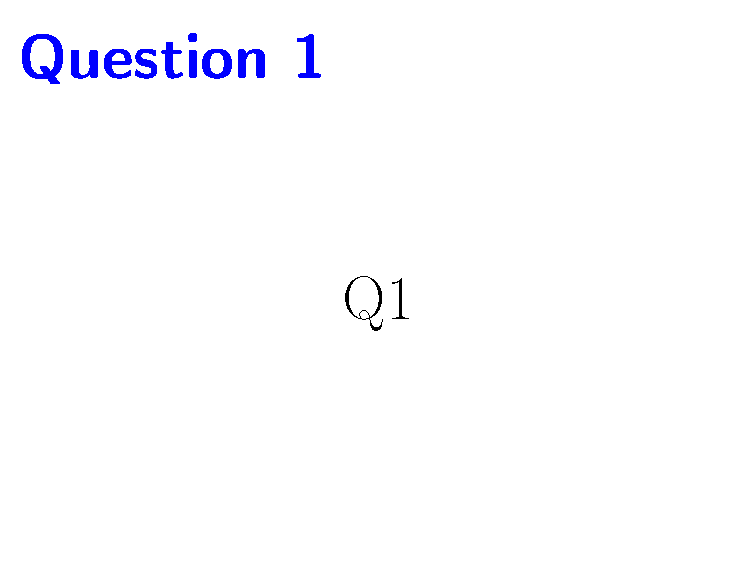
\includegraphics[height=4cm]{documentation_res/beamerq}}
        
        \vspace{2pt}
    \end{center}
\end{minipage}
\hfill\vline\hrule
\footnotetext{Cette commande doit être utilisée entre \mintinline{latex}?\begin{document}? et \mintinline{latex}?\end{document}?}
\vline\hfill
\begin{minipage}{0.475\linewidth}
    \begin{center}
        \vspace{2pt}
        \mintinline{latex}?\slider{R1}{1}?\footnotemark

        \vspace{2pt}
    \end{center}
\end{minipage}
\hfill\vline\hfill
\begin{minipage}{0.475\linewidth}
    \begin{center}
        \vspace{2pt}
        \fbox{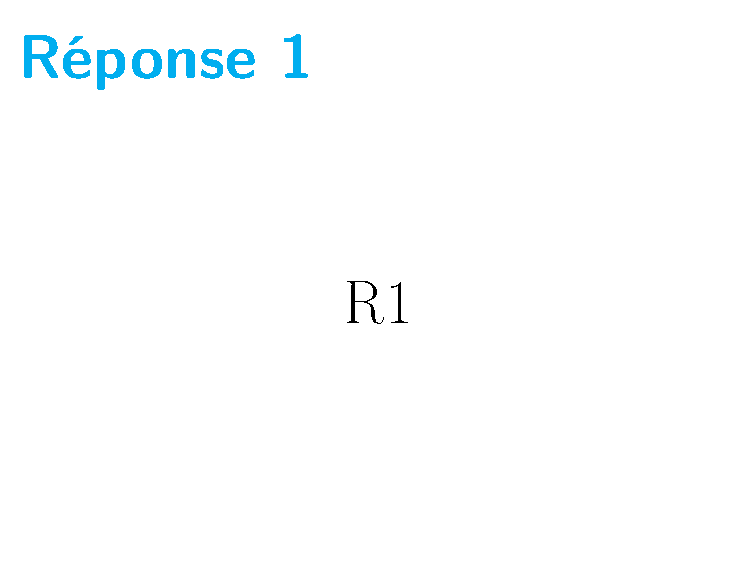
\includegraphics[height=4cm]{documentation_res/beamerr}}
        
        \vspace{2pt}
    \end{center}
\end{minipage}
\hfill\vline\hrule
\footnotetext{Cette commande doit être utilisée entre \mintinline{latex}?\begin{document}? et \mintinline{latex}?\end{document}?}
\hsection{AL.sty}
Le package \hyperlink{section.10}{\texttt{Matrices.sty}} sera importé automatiquement avec \texttt{AL.sty}.

\vspace{0.5cm}

\mhd
\mcmd{\oldvect}
\mcmd{\vect{E}}
\mcmd{\al{E}{}}
\mcmd{\al{E}{F}}
\mcmd[\footnotemark]{\oplus}
\footnotetext{Le \mintinline{latexmath}?\oplus? utilisé est celui de \href{https://ctan.org/pkg/stmaryrd}{\color{black}\texttt{stmaryrd}}\\Pour récupérer celui de \LaTeX, il est possible d'utiliser la commande \mintinline{latex}?\let\oldoplus\oplus? avant \mintinline{latex}?\usepackage{al}? puis de faire \mintinline{latex}?\let\oplus\oldoplus? après importation\\Comparaison \LaTeX~- \href{https://ctan.org/pkg/stmaryrd}{\color{black}\texttt{stmaryrd}} avec le plus normal $\oldoplus\oplus+$}
\mcmd[\footnotemark]{\matgl{n}{\mathbb{K}}}
\footnotetext{Le \mintinline{latexmath}?\matgl? de \texttt{AL.sty} correspond à la commande \mintinline{latexmath}?\gl? de \hyperlink{section.10}{\texttt{Matrices.sty}} qui a été renommé}
\mcmd{\gl{E}}
\mcmd[\footnotemark]{\olddim}
\footnotetext{Correspond à la commande usuelle \mintinline{latexmath}?\dim?}
\mcmd{\dim{E}}
\mcmd{\oldrg}
\mcmd{\rg{u}}
\mcmd{\oldtr}
\mcmd{\tr{u}}
\mcmd{\oldmat}
\mcmd[\footnotemark]{\almat{u}{\mathcal{B}}{}}
\footnotetext{Ne pas confondre cette commande avec \mintinline{latexmath}?\mat? de \hyperlink{section.10}{\texttt{Matrices.sty}}}
\mcmd{\almat{u}{\mathcal{B}}{\mathcal{C}}}
\mmcmd[\footnotemark]{\lc}{$\lc\right.$}
\footnotetext{Correspond à la commande usuelle \mintinline{latexmath}?\left[?}
\mmcmd[\footnotemark]{\rc}{$\left.\rc$}
\footnotetext{Correspond à la commande usuelle \mintinline{latexmath}?\right]?}
\mcmd{\oldsl}
\mcmd{\sl{E}}
\mcmd{\sl[n]{\mathbb{K}}}
\mcmd{\oldorth}
\mcmd{\orth{n}}
\mcmd{\orth[n]{\mathbb{R}}}
\mcmd{\oldso}
\mcmd{\so{n}}
\mcmd{\so[n]{\mathbb{R}}}
\hsection{Analyse.sty}
Le package \hyperlink{section.6}{\texttt{BigOperators.sty}} sera importé automatiquement avec \texttt{Analyse.sty}.

\vspace{0.5cm}

\mhd
\mcmd[\footnotemark]{\dd}
\footnotetext{$\dd$ de dérivation}
\mcmd{\der{}{f(x)}}
\mcmd{\der[n]{}{f(x)}}
\mcmd{\der[][t]{f(t)}{}}
\mcmd[\footnotemark]{\der[n][t]{f}{t}}
\footnotetext{Le parenthésage de l'expression dans le second argument se fait automatiquement si ce dernier est non vide}
\mcmd[\footnotemark]{\pder{}{f(x,y)}}
\footnotetext{On peut appliquer les mêmes arguments optionnels que pour \mintinline{latexmath}?\der? et les arguments obligatoires sont les mêmes que pour \mintinline{latexmath}?\der?}
\mcmd[\footnotemark]{\mpder[x,y,z]{}{f(x,y,z)}}
\footnotetext{Sans argument optionnel, \mintinline{latexmath}?\mpder? agit comme \mintinline{latexmath}?\pder? et les arguments obligatoires sont les mêmes que pour \mintinline{latexmath}?\der?}
\mcmd[\footnotemark]{\mpder[x_1,x_2,x_3,x_3]{f(X)}{}}
\footnotetext{\mintinline{latexmath}?\mpder? peut ne pas marcher avec des variables de plusieurs lettres\\Si la commande n'affiche pas le résultat attendu avec des variabled de plusieurs lettres, il faut utiliser \mintinline{latex}?\usepackage[dvar]{analyse}?\\Cette option importe automatiquement \texttt{pgffor} (qui est utilisé importé par \tikzlg{} et PGF)}
\mcmd[\footnotemark]{\oldint}
\footnotetext{Correspond à la commande usuelle \mintinline{latexmath}?\int?}
\mcmd{\int{f}}
\mcmd{\int[t]{f(t)}}
\mcmd[\footnotemark]{\int[t][{[a,b]}]{f(t)}}
\footnotetext{L'argument \mintinline{latexmath}?[a,b]? doit être mis entre accolades pour être traîté correctement par \LaTeX}
\mcmd{\int[t][a][b]{f(t)}}
\mcmd{\int[][a][b]{f'}}
\mcmd{\eval[{[a,b]}]{f(t)}}
\mcmd{\eval[a][b]{f(t)}}
\pagebreak
\hrule
\mcmd[\footnotemark]{\serie{a_n}}
\footnotetext{Comme \hyperlink{section.6}{\texttt{BigOperators.sty}} est chargé, la commande \mintinline{latexmath}?\sum? est remplacée et il est nécessaire de taper \mintinline{latexmath}?\oldsum? pour obtenir $\oldsum$}
\mcmd{\oldesc}
\mcmd{\esc{\left[a,b\right]}}
\mcmd{\esc[+]{f}}
\mcmd{\nrm{f}}
\mcmd{\nrm[1]{g}}
\mcmd{\oldva}
\mcmd{\va{u}}
\mcmd{\oldepi}
\mcmd{\epi{f}}
\hsection{Arithmetique.sty}
\mhd
\mcmd[\footnotemark]{\olddiv}
\footnotetext{Correspond à la commande usuelle \mintinline{latexmath}?\div?}
\mcmd[\footnotemark]{\div}
\footnotetext{Correspond à la commande usuelle \mintinline{latexmath}?\mid?}
\mcmd{\cgr{a}{b}{n}}
\mcmd[\footnotemark]{\oldphi}
\footnotetext{Correspond à la commande usuelle \mintinline{latexmath}?\phi?}
\mcmd[\footnotemark]{\phi}
\footnotetext{Correspond à la commande usuelle \mintinline{latexmath}?\varphi?}
\hsection{BigOperators.sty}
\mhd
\mcmd[\footnotemark]{\oldsum}
\footnotetext{Correspond à la commande usuelle \mintinline{latexmath}?\sum?}
\mcmd{\sum{n=0}{+\infty}{u_n}}
\mcmd[\footnotemark]{\oldprod}
\footnotetext{Correspond à la commande usuelle \mintinline{latexmath}?\prod?}
\mcmd{\prod{n=0}{+\infty}{u_n}}
\mcmd[\footnotemark]{\oldcap}
\footnotetext{Correspond à la commande usuelle \mintinline{latexmath}?\bigcap?}
\mcmd{\bigcap{n=0}{+\infty}{A_n}}
\mcmd[\footnotemark]{\oldcup}
\footnotetext{Correspond à la commande usuelle \mintinline{latexmath}?\bigcup?}
\mcmd{\bigcup{n=0}{+\infty}{A_n}}
\mcmd[\footnotemark]{\olduplus}
\footnotetext{Correspond à la commande usuelle \mintinline{latexmath}?\biguplus?}
\mcmd{\biguplus{n=0}{+\infty}{A_n}}
\mcmd{\bigop{n=0}{+\infty}{E_n}}
\hsection{Complexes.sty}
\mhd
\mcmd[\footnotemark]{\oldbar{z}}
\footnotetext{Correspond à la commande usuelle \mintinline{latexmath}?\bar?}
\mcmd[\footnotemark]{\bar{z}}
\footnotetext{Se comporte comme \mintinline{latexmath}?\overline?}
\mcmd[\footnotemark]{\e}
\footnotetext{$\e$ de la fonction exponentielle}
\mcmd[\footnotemark]{\i}
\footnotetext{$\i$ complexe\\L'ancienne commande \mintinline{latex}?\i? s'obtient avec \mintinline{latex}?\ii?}
\mcmd[\footnotemark]{\j}
\footnotetext{$\j=\e^{\oldfrac{2\i\pi}{3}}$\\L'ancienne commande \mintinline{latex}?\j? s'obtient avec \mintinline{latex}?\jj?}
\mcmd[\footnotemark]{\oldIm}
\footnotetext{Correspond à la commande usuelle \mintinline{latexmath}?\Im?}
\mcmd{\Im}
\mcmd{\pIm{x}}
\mcmd[\footnotemark]{\oldRe}
\footnotetext{Correspond à la commande usuelle \mintinline{latexmath}?\Re?}
\mcmd{\Re}
\mcmd{\pRe{x}}
\subsection{Dessiner des arcs}
Il est aussi possible de faire des arcs en important le package \texttt{Complexes.sty} avec l'option {\color{namecolour}\texttt{arc}}, en utilisant \mintinline{latex}?\usepackage[arc]{complexes}? au lieu de \mintinline{latex}?\usepackage{complexes}?.

Cette option importe automatiquement le package \texttt{graphics} (disponible sur \href{https://ctan.org/pkg/graphics}{CTAN}).
\vspace{0.5cm}
\mhd
\mcmd{\arc{AB}}
\mcmd{\arc{ABCDEFFGH}}
\hsection{Dsft.sty}
Ce package remplace le $\mathds 1$ du package \texttt{Dsfonts.sty} disponible sur \href{https://www.ctan.org/pkg/doublestroke}{CTAN} et introduit quelques symboles.

\vspace{0.5cm}

\mhd
\mcmd{\mathds{1}}
\mcmd{\1{E}(x)}
\mcmd{\square}
\mcmd{\star}
\mcmd{\triangle}
\subsection{\href{https://rfoxinter.github.io/revisions/output/dsrom12.pfb}{\color{black}\texttt{dsrom12.pfb}} et \href{https://rfoxinter.github.io/revisions/output/dsrom12.tfm}{\color{black}\texttt{dsrom12.tfm}}}

Pour utiliser ce package, il faut copier les fichiers \texttt{dsrom12.pfb} et \texttt{dsrom12.tfm} dans les dossiers où ils sont actuellement avec \texttt{dsfonts} (et éventuellement créer une copie des anciens fichiers).
\hsection{Equivalents.sty}
\mhd
\mcmd{\o{x}}
\mcmd{\o[x\to0]{x}}
\mcmd{\O{x}}
\mcmd{\O[x\to0]{x}}
\mcmd{\Th{x}}
\mcmd{\Th[x\to0]{x}}
\mcmd{\Om{x}}
\mcmd{\Om[x\to0]{x}}
\mcmd{\eq{u_n}{v_n}}
\mcmd{\eq[n\to+\infty]{u_n}{v_n}}
\mcmd{\eg{u_n}{v_n+\o{v_n}}}
\mcmd{\eg[n\to+\infty]{u_n}{v_n+\o{v_n}}}
\hsection{Matrices.sty}
\mhd
\mcmd{\mat{n}{p}{\mathbb{K}}}
\mcmd{\mat{n}{}{\mathbb{K}}}
\mcmd{\sym{n}{\mathbb{K}}}
\mcmd{\ant{n}{\mathbb{K}}}
\mcmd{\diag{n}{\mathbb{K}}}
\mcmd{\ts{n}{\mathbb{K}}}
\mcmd{\ti{n}{\mathbb{K}}}
\mcmd[\footnotemark]{\olddet}
\footnotetext{Correspond à la commande usuelle \mintinline{latexmath}?\det?}
\mcmd{\det{M}}
\mcmd{\det[\mathcal{B}]{\mathcal{B}'}}
\mcmd{\oldgl}
\mmcmd[\footnotemark]{\gl{n}{\mathbb{K}}}{$\matgl{n}{\mathbb{K}}$}
\footnotetext{Si \texttt{AL.sty} est chargé, cette commande est remplacée et il faut utiliser \mintinline{latexmath}?\matgl{n}{\mathbb{K}}? pour obtenir ce résultat}
\mcmd{\oldcom}
\mcmd{\com{M}}
\mmcmd{\mdots}{$\oldmdots$}
\mmcmd{\ddots}{$\oldddots$}
\mmcmd{\idots}{$\oldidots$}
\mmcmd{\vdots}{$\oldvdots$}
\mmcmd{\xdots}{$\oldxdots$}
\mmcmd{\plusdots}{$\oldplusdots$}
\mcmd[\footnotemark]{\tmatrix({1\&0\\0\&1\\})}
\footnotetext{Les caractères \mintinline{latex}?\&? sont utilisés au lieu du \mintinline{latex}?&? utilisé habituellement avec \tikzlg{} pour des raisons de compatibilité avec \href{https://ctan.org/pkg/beamer}{\color{black}\textsc{beamer}}\\Il n'est pas nécessaire de mettre la \mintinline{latex}?\tmatrix? dans une équation et les cellules sont par défaut des équations}
\subsection{\boldmath Ne pas importer les commandes avec $\mcdot$}
Il est possible de ne pas modifier les commandes usuelles en utilisant l'option {\color{namecolour}\texttt{nodots}} de ce package. Il faut alors importer le package avec \mintinline{latex}?\usepackage[nodots]{matrices}?.
\subsection{\boldmath Modifier les séparations entre les $\mcdot$}
Les commandes avec des points tel que $\xdots$ ont des définitions qui dépendent de la taille de la police. Par défaut, celle pour \LaTeX~est adaptée pour 12pt, et celle de \href{https://ctan.org/pkg/beamer}{\color{black}\textsc{beamer}} pour 17pt. Pour avoir des points alignés correctement, il est possible de modifier la valeur de \mintinline{latex}?\dotsep? en utilisant \mintinline{latex}?\setlength{\dotsep}{Xpt}?.

Par exemple, avec 2pt, on obtient : \setlength{\dotsep}{2pt}<< $\xdots$ >>.\setlength{\dotsep}{3.5pt}

Il est également possible de faire de même avec la hauteur des $\mdots$ en modifiant la longueur \mintinline{latex}?\dotlift?. De même avec \mintinline{latex}?\matmin? pour {\color{namecolour}\texttt{minimum width}} et {\color{namecolour}\texttt{minimum width}}, ou encore \mintinline{latex}?\matsep? pour {\color{namecolour}\texttt{row sep}} et {\color{namecolour}\texttt{column sep}}.
\subsection{La commande \mintinline{latex}?\tmatrix?}

\mintinline{latex}?\tmatrix? est composé de deux arguments optionnels (les éléments à ajouter à la matrice \tikzlg{} et les éléments de mise en page de la matrice) ainsi que de trois arguments (le délimiteur d'ouverture, le contenu de la matrice et le délimiteur de fermeture).

\vspace{0.5cm}

\mhd
\nmcmd{\mtxvline{params}{n}}{Crée une ligne verticale après la colonne \texttt{n} (ou \texttt{left}/\texttt{right} pour les extrémités) avec les paramètres \tikzlg{} \texttt{params}}
\nmcmd{\mtxhline{params}{n}}{Crée une ligne horizontale après la ligne \texttt{n} (ou \texttt{top}/\texttt{bottom} pour les extrémités) avec les paramètres \tikzlg{} \texttt{params}}
\nmcmd{\mtxvpartial{params}{n}{a}{b}}{Crée une ligne verticale après la colonne \texttt{n} (ou \texttt{left}/\texttt{right} pour les extrémités), la ligne ayant pour extrémités la fin de la ligne \texttt{a} et \texttt{b} (ou \texttt{top}/\texttt{bottom}) avec les paramètres \tikzlg{} \texttt{params}}
\nmcmd{\mtxhpartial{params}{n}{a}{b}}{Crée une ligne horizontale après la ligne \texttt{n} (ou \texttt{top}/\texttt{bottom} pour les extrémités), la ligne ayant pour extrémités la fin de la ligne \texttt{a} et \texttt{b} (ou \texttt{left}/\texttt{right}) avec les paramètres \tikzlg{} \texttt{params}}
\nmcmd{\mtxbox{params}{x}{y}}{Crée une boîte autour de la case de coordonnées \texttt{x} et \texttt{y} (l'indexation commence à 1) avec les paramètres \tikzlg{} \texttt{params}}
\subsection{Exemples avec \mintinline{latex}?\tmatrix?}

$\det M=\tmatrix|{a\&b\\c\&d\\}|$ est produit par \mintinline{latex}?$\det{M}=\tmatrix|{a\&b\\c\&d\\}|$?.

\vspace{0.25cm}

$I_{n,p,r}=\tmatrix[\mtxvline{line width = 0.05em}{1}\mtxhline{line width = 0.05em}{1}][minimum height = 5ex, row sep = 1ex,minimum width = 5ex, column sep = 1ex,]({I_r\&0_{r,p-r}\\0_{n-r,r}\&0_{n-r,p-r}\\})$ est produit par
\vspace{-\abovedisplayskip}\begin{minted}{latex}
$
I_{n,p,r}=\tmatrix
    [\mtxvline{line width = 0.05em}{1}\mtxhline{line width = 0.05em}{1}]
    [minimum height = 5ex, row sep = 1ex, minimum width = 5ex,
        column sep = 1ex,]
    ({I_r\&0_{r,p-r}\\0_{n-r,r}\&0_{n-r,p-r}\\})
$
\end{minted}
\vspace{-\belowdisplayskip}

\vspace{0.25cm}

\tmatrix[\mtxbox{red, dashed}{1}{1}\mtxbox{teal, dotted, ultra thick}{2}{2}\mtxbox{}{4}{4}][minimum height = 5ex, minimum width = 5ex, row sep = 10pt,inner sep = 5pt, column sep = 10pt,]{{[}}{A_1\&0\&0\&0\\0\&A_2\&\ddots\&0\\0\&\ddots\&\ddots\&0\\0\&0\&0\&A_n\\}{\}} est produit par
\vspace{-\abovedisplayskip}\begin{minted}[breaklines,breakafter=\&,breakaftersymbolpre=,breaksymbol=~~~~,curlyquotes]{latex}
\tmatrix
    [
        \mtxbox{red, dashed}{1}{1}
        \mtxbox{teal, dotted, ultra thick}{2}{2}
        \mtxbox{}{4}{4}
    ]
    [
        minimum height = 5ex,
        minimum width = 5ex,
        row sep = 10pt,
        inner sep = 5pt,
        column sep = 10pt,
    ]
    {{[}} % Le crochet est entouré de deux paires d'accolades
    {
        A_1\&0\&0\&0\\
        0\&A_2\&\ddots\&0\\
        0\&\ddots\&\ddots\&0\\
        0\&0\&0\&A_n\\
    }
    {\}}
\end{minted}
\vspace{-\belowdisplayskip}
\hsection{Polynomes.sty}
\mhd
\mcmd{\pol{K}{X}}
\mcmd{\fr{K}{X}}
\mcmd[\footnotemark]{\olddeg}
\footnotetext{Correspond à la commande usuelle \mintinline{latexmath}?\deg?}
\mcmd{\deg{P}}
\mcmd{\oldval}
\mcmd{\val{P}}
\mcmd{\oldcar}
\mcmd{\car{\mathbb{K}}}
\hsection{Probas.sty}
\mhd
\mcmd{\p{A}}
\mcmd{\p[B]{A}}
\mcmd[\footnotemark]{\oldOmega}
\footnotetext{Correspond à la commande usuelle \mintinline{latexmath}?\Omega?}
\mcmd[\footnotemark]{\Omega}
\footnotetext{Correspond à la commande usuelle \mintinline{latexmath}?\varOmega?}
\mmcmd[\footnotemark]{\sq}{$\left.\sq\right.$}
\footnotetext{Correspond à la commande usuelle \mintinline{latexmath}?\middle|?\\Doit être utilisé entre \mintinline{latexmath}?\left? et \mintinline{latexmath}?\right?, ou dans la commande \mintinline{latexmath}?\p?: $\p{A\sq\bigcap{k=1}{n}{B_i}}$}
\mcmd[\footnotemark]{\bor}
\footnotetext{Correspond à la commande usuelle \mintinline{latexmath}?\mathcal{B}?}
\mcmd{\esp{X}}
\mcmd{\var{X}}
\mcmd{\ect{X}}
\mcmd{\oldcov}
\mcmd{\cov{X}{Y}}
\mcmd[\footnotemark]{\indep}
\footnotetext{Ce symbole est obtenu avec la commande \mintinline{latexmath}?\perp\!\!\!\perp?}
\mcmd{\unif{n}}
\mcmd{\bin{p}}
\mcmd{\bin[n]{p}}
\mcmd{\geom{p}}
\mcmd{\pasc{r}{p}}
\mcmd{\nbin{r}{p}}
\mcmd{\hypg{N}{n}{q}}
\mcmd{\poiss{\lambda}}
\hsection{Sffont.sty}
Ce package définit une nouvelle police \texttt{cmssp} qui correspond à \texttt{cmss} en 10pt. Pour l'utiliser, il faut utiliser \mintinline{latex}?\fontfamily{cmssp}\fontsize{Xpt}{\baselineskip}\selectfont?.

\vspace{0.5cm}

Comparaison entre \texttt{cmssp} et \texttt{cmss} :

\hrule\vline\hfill
\begin{minipage}{0.475\linewidth}
    \begin{center}
        \vspace{2pt}
        \texttt{cmssp}

        \vspace{2pt}
    \end{center}
\end{minipage}
\hfill\vline\hfill
\begin{minipage}{0.475\linewidth}
    \begin{center}
        \vspace{2pt}
        \texttt{cmss}
        
        \vspace{2pt}
    \end{center}
\end{minipage}
\hfill\vline\hrule
\mln{{\bfseries\fontfamily{cmssp}\fontsize{21pt}{\baselineskip}\selectfont Exemple avec une police de taille 21pt en gras.}}{{\bfseries\fontfamily{cmss}\fontsize{21pt}{\baselineskip}\selectfont Exemple avec une police de taille 21pt en gras.}}
\mln{{\itshape\fontfamily{cmssp}\fontsize{17pt}{\baselineskip}\selectfont Exemple avec une police de taille 17pt en italique.}}{{\itshape\fontfamily{cmss}\fontsize{17pt}{\baselineskip}\selectfont Exemple avec une police de taille 17pt en italique.}}
\mln{{\itshape\bfseries\fontfamily{cmssp}\fontsize{12pt}{\baselineskip}\selectfont Exemple avec une police de taille 12pt en gras italique.}}{{\itshape\bfseries\fontfamily{cmss}\fontsize{12pt}{\baselineskip}\selectfont Exemple avec une police de taille 12pt en gras italique.}}
\hsection{Structures.sty}
\mhd
\mcmd{\oldhom}
\mcmd{\hom{E}}
\mcmd{\oldaut}
\mcmd{\aut{E}}
\mcmd[\footnotemark]{\oldker}
\footnotetext{Correspond à la commande usuelle \mintinline{latexmath}?\ker?}
\mcmd{\ker{f}}
\mcmd{\oldim}
\mcmd{\im{f}}
\mmcmd[\footnotemark]{\la}{$\la\right.$}
\footnotetext{Correspond à la commande usuelle \mintinline{latexmath}?\left\langle?}
\mmcmd[\footnotemark]{\ra}{$\left.\ra$}
\footnotetext{Correspond à la commande usuelle \mintinline{latexmath}?\right\rangle?}
\mcmd{\oldord}
\mcmd{\ord{x}}
\hsection{Tables.sty}
Ce package sert à mettre en forme des tables an latex grâce à \tikzlg{}.

Pour insérer une table, il faut appeler \mintinline{latex}?\setrowcol[width][height]{ncols}{nrows}? avec le nombre de colonnes et de lignes de la table, puis rentrer la table \tikzlg{}, les arguments optionnels étant la largeur de la table et sa hauteur.

Une table a une largeur par défaut de 10cm et une hauteur de 6,5cm (est est réinitialisée à chaque appel de \mintinline{latex}?\setrowcol?).

Il est possible d'utiliser \mintinline{latex}?[ampersand replacement=\&]? puis \mintinline{latex}?\&? pour la matrice lorsque \mintinline{latex}?&? est déjà défini par l'environnement (comme \textsc{beamer}).

Il est possible de récupérer la valeur de la largeur et de la hauteur avec \mintinline{latex}?\tblw? et \mintinline{latex}?\tblh?.

\vspace{0.5cm}

Par exemple, la table

\vspace{-\abovedisplayskip}\begin{center}
{\LARGE\setcolrow[15cm]{6}{5}\begin{tikzpicture}\matrix[table]{&$0$&$\oldfrac{\pi}{6}$&$\oldfrac{\pi}{4}$&$\oldfrac{\pi}{3}$&$\oldfrac{\pi}{2}$ \\ $\oldsin$&$0$&$\oldfrac{1}{2}$&$\oldfrac{\sqrt{2}}{2}$&$\oldfrac{\sqrt{3}}{2}$&$1$\\ $\oldcos$&$1$&$\oldfrac{\sqrt{3}}{2}$&$\oldfrac{\sqrt{2}}{2}$&$\oldfrac{1}{2}$&$0$\\ $\oldtan$&$0$&$\oldfrac{1}{\sqrt{3}}$&$1$&$\sqrt{3}$&--\\ $\oldcot$&--&$\sqrt{3}$&$1$&$\oldfrac{1}{\sqrt{3}}$&$0$\\}; \draw [line width=0.5mm] (-\tblw/3,-\tblh/2) -- (-\tblw/3,\tblh/2); \draw [line width=0.5mm] (-\tblw/2,3*\tblh/10) -- (\tblw/2,3*\tblh/10); \draw [line width=0.5mm] (-\tblw/2,-\tblh/2) rectangle (\tblw/2,\tblh/2);\end{tikzpicture}}
\end{center}
\vspace{-\belowdisplayskip}
est produite avec le code suivant
\vspace{-\abovedisplayskip}\begin{minted}[breaklines,breakafter=&,breakaftersymbolpre=,breaksymbol=~~~~]{latex}
\LARGE
\setcolrow[15cm]{6}{5}
\begin{tikzpicture}
    \matrix[table]{
        &$0$&$\oldfrac{\pi}{6}$&$\oldfrac{\pi}{4}$&$\oldfrac{\pi}{3}$&$\oldfrac{\pi}{2}$\\
        $\oldsin$&$0$&$\oldfrac{1}{2}$&$\oldfrac{\sqrt{2}}{2}$&$\oldfrac{\sqrt{3}}{2}$&$1$\\
        $\oldcos$&$1$&$\oldfrac{\sqrt{3}}{2}$&$\oldfrac{\sqrt{2}}{2}$&$\oldfrac{1}{2}$&$0$\\
        $\oldtan$&$0$&$\oldfrac{1}{\sqrt{3}}$&$1$&$\sqrt{3}$&--\\
        $\oldcot$&--&$\sqrt{3}$&$1$&$\oldfrac{1}{\sqrt{3}}$&$0$\\
    };
    \draw [line width=0.5mm] (-\tblw/3,-\tblh/2) -- (-\tblw/3,\tblh/2);
    \draw [line width=0.5mm] (-\tblw/2,3*\tblh/10) -- (\tblw/2,3*\tblh/10);
    \draw [line width=0.5mm] (-\tblw/2,-\tblh/2) rectangle (\tblw/2,\tblh/2);
\end{tikzpicture}
\end{minted}
\vspace{-\belowdisplayskip}
\hsection{Tools.sty}
Ce fichier fournit des commandes latex utiles pour créer des macros.

\vspace{0.5cm}

\mhd
\nmcmd{\comparestring{a}{b}{if}{else}}{Compare les chaînes de caractères \mintinline{latex}?a? et \mintinline{latex}?b?; puis exécute le \mintinline{latex}?if? si \mintinline{latex}?a? est égal à \mintinline{latex}?b? et le \mintinline{latex}?else? sinon}
\hsection{Trigo.sty}
\mhd
\mcmd[\footnotemark]{\oldcos}
\footnotetext{Correspond à la commande usuelle \mintinline{latexmath}?\cos?}
\mcmd{\cos{x}}
\mcmd{\cos[n]{x}}
\mcmd[\footnotemark]{\oldsin}
\footnotetext{Correspond à la commande usuelle \mintinline{latexmath}?\sin?}
\mcmd{\sin{x}}
\mcmd{\sin[n]{x}}
\mcmd[\footnotemark]{\oldtan}
\footnotetext{Correspond à la commande usuelle \mintinline{latexmath}?\tan?}
\mcmd{\tan{x}}
\mcmd{\tan[n]{x}}
\mcmd[\footnotemark]{\oldcot}
\footnotetext{Correspond à la commande usuelle \mintinline{latexmath}?\cot?}
\mcmd{\cot{x}}
\mcmd{\cot[n]{x}}
\mcmd{\acos{x}}
\mcmd{\acos[n]{x}}
\mcmd{\asin{x}}
\mcmd{\asin[n]{x}}
\mcmd{\atan{x}}
\mcmd{\atan[n]{x}}
\mcmd{\oldch}
\mcmd{\ch{x}}
\mcmd{\ch[n]{x}}
\mcmd{\oldsh}
\mcmd{\sh{x}}
\mcmd{\sh[n]{x}}
\mcmd{\oldth}
\mcmd{\th{x}}
\mcmd{\th[n]{x}}
\mcmd{\oldach}
\mcmd{\ach{x}}
\mcmd{\ach[n]{x}}
\mcmd{\oldash}
\mcmd{\ash{x}}
\mcmd{\ash[n]{x}}
\mcmd{\oldath}
\mcmd{\ath{x}}
\mcmd{\ath[n]{x}}
\hsection{Usuelles.sty}
\mhd
\mcmd[\footnotemark]{\oldmin}
\footnotetext{Correspond à la commande usuelle \mintinline{latexmath}?\min?}
\mcmd{\min{\llb0,n\rrb}}
\mcmd{\min[\mathbb{N}^*]{\llb0,n\rrb}}
\mcmd[\footnotemark]{\oldmax}
\footnotetext{Correspond à la commande usuelle \mintinline{latexmath}?\max?}
\mcmd{\max{\llb0,n\rrb}}
\mcmd{\max[\mathbb{Z}_-]{\llb0,n\rrb}}
\mcmd[\footnotemark]{\oldlim}
\footnotetext{Correspond à la commande usuelle \mintinline{latexmath}?\lim?}
\mcmd{\lim{u_n}}
\mcmd{\lim[x\to+\infty]{f(x)}}
\mcmd{\limi{u_n}}
\mcmd{\limi[x\to+\infty]{f(x)}}
\mcmd{\lims{u_n}}
\mcmd{\lims[x\to+\infty]{f(x)}}
\mcmd[\footnotemark]{\oldexp}
\footnotetext{Correspond à la commande usuelle \mintinline{latexmath}?\exp?}
\mcmd{\exp{x}}
\mcmd{\exp[n]{x}}
\mcmd[\footnotemark]{\oldln}
\footnotetext{Correspond à la commande usuelle \mintinline{latexmath}?\ln?}
\mcmd{\ln{x}}
\mcmd{\ln[n]{x}}
\mcmd[\footnotemark]{\oldinf}
\footnotetext{Correspond à la commande usuelle \mintinline{latexmath}?\inf?}
\mcmd{\inf{\varnothing}}
\mcmd{\inf[\bar{\mathbb{R}}]{\{u_n\}}}
\mcmd[\footnotemark]{\oldsup}
\footnotetext{Correspond à la commande usuelle \mintinline{latexmath}?\sup?}
\mcmd{\sup{\varnothing}}
\mcmd{\sup[\bar{\mathbb{R}}]{\{u_n\}}}
\end{document}
